%-----------------------------------------------------------------------------%
\chapter{\babEnam}
%-----------------------------------------------------------------------------%

In this chapter, the \verb|JSONField| implementation explained in the fourth
chapter is evaluated on all of the database systems supported by Django.

%-----------------------------------------------------------------------------%
\section{Tests}
%-----------------------------------------------------------------------------%

To ensure that the behavior of \verb|JSONField| is consistent across all of the
database systems supported by Django, existing tests for the PostgreSQL-only
implementation are run for other database systems as well. The tests were
gradually moved from the \verb|postgres_tests| directory to the
\verb|model_fields| and \verb|form_tests/field_tests| directories during
development. By moving the tests outside of \verb|postgres_tests| and modifying
the test classes to use the new implementation, the tests can now be run on
other database systems.

\begin{table}
	\centering
\begin{tabular}{|c|l|c|p{6.6cm}|}
\hline
No. & Test class                  & No. of tests & Test cases description \\ \hline
1.  & \texttt{JSONFieldTests}     & 3            & Non-serializable value, custom encoder and decoder usage, and database check constraints. \\ \hline
2.  & \texttt{TestMethods}        & 4            & \texttt{deconstruct()}, \texttt{get\_transforms()}, etc. \\ \hline
3.  & \texttt{TestValidation}     & 4            & Invalid encoder and decoder, invalid JSON value, etc. \\ \hline
4.  & \texttt{TestFormField}      & 2            & \texttt{formfield()} with and without custom encoder and decoder. \\ \hline
5.  & \texttt{TestSerialization}  & 2            & Serialization and deserialization with Django's serialization framework. \\ \hline
6.  & \texttt{TestSaveLoad}  	  & 6            & Saving and loading various JSON data. \\ \hline
7.  & \texttt{TestQuerying}       & 49           & Querying various JSON data with different scenarios (including lookups and transforms). \\ \hline
\end{tabular}
\caption{The \code{JSONField} model field test classes and their descriptions.}
\label{table:testclasses}
\end{table}

The tests for \verb|JSONField| are split into different files according to
Django's test files structure. The majority of the tests are written in the
\verb|model_fields.test_jsonfield| module, which consists of 70 test cases
divided into 7 test classes, as shown by \autoref{table:testclasses}. As seen
in the table, the \verb|JSONField| querying functionalities have the largest
number of tests for different querying scenarios. In addition to tests from the
previous PostgreSQL-only implementation, the \verb|JSONField| tests also
include new tests for new features and documented behaviors.

Aside from the tests specific to the model field, there are also tests for the
other parts of the ORM as well as the form field. The tests for the other ORM
parts include tests for system checks in regards to \verb|JSONField| support on
the database backends, tests for default value in \verb|JSONField|, tests for
\verb|JSONField| casting operations, and others. These tests are written in
separate modules, i.e. the \verb|test_models| and \verb|test_ordinary_fields|
modules in the \verb|invalid_models_tests| module, the
\verb|backends.base.test_operations| module, etc. Meanwhile, the form field
tests are written in the \verb|form_tests.field_tests.test_jsonfield| module,
which consists of 12 test cases in a single test class.

\listing
{Python}
{The \code{test\_custom\_encoder\_decoder()} test method.}
{code:testencodecoder}
{codes/6-testencodecoder.py}

One of the new tests is \verb|test_custom_encoder_decoder()| shown by
\autoref{code:testencodecoder}. The test is modified from
\verb|test_custom_encoder()| in the PostgreSQL-only implementation, which does
not support a custom decoder. The test describes the process of creating a
\verb|NullableJSONModel| object that contains a \verb|UUID| object inside a
\verb|JSONField| (lines 3 and 4). The \verb|NullableJSONModel| class is a model
class (for \verb|JSONField| tests) that has a \verb|JSONField| named
\verb|value_custom| that is equipped with custom encoder and decoder.  Upon
cleaning the fields (line 5) and saving the object to the database (line 6),
the object is retrieved (refreshed) from the database (line 7). The retrieved
object is asserted to be equal to the initial object (line 8), which means that
the JSON object is successfully deserialized to retain the \verb|UUID| object.
The deserialization is only possible if a custom decoder is used because the
default decoder does not provide deserialization to \verb|UUID| objects.

\listing
{Python}
{The \code{test\_json\_null\_different\_from\_sql\_null()} test method.}
{code:testnull}
{codes/6-testnull.py}

The \verb|test_json_null_different_from_sql_null()| method shown by
\autoref{code:testnull} is another example of the new tests. The test verifies
the \verb|JSONField| behavior with JSON \verb|null| and SQL \verb|NULL| values,
which was not documented in the PostgreSQL-only implementation. The test works
by using JSON \verb|null| and SQL \verb|NULL| values to create model objects
that are assigned to \verb|json_null| and \verb|sql_null| variables,
respectively (lines 5 and 7). After refreshing both objects (lines 6 and 8),
queries for the JSON \verb|null| value is verified using \verb|Value('null')|
and \verb|None| (lines 10 to 17). Meanwhile, the SQL \verb|NULL| value is
verified by using the \verb|isnull| lookup (lines 18 to 21). Finally, both
values are asserted to be equal in Python, i.e. \verb|None|.

\begin{figure}
	\centering
    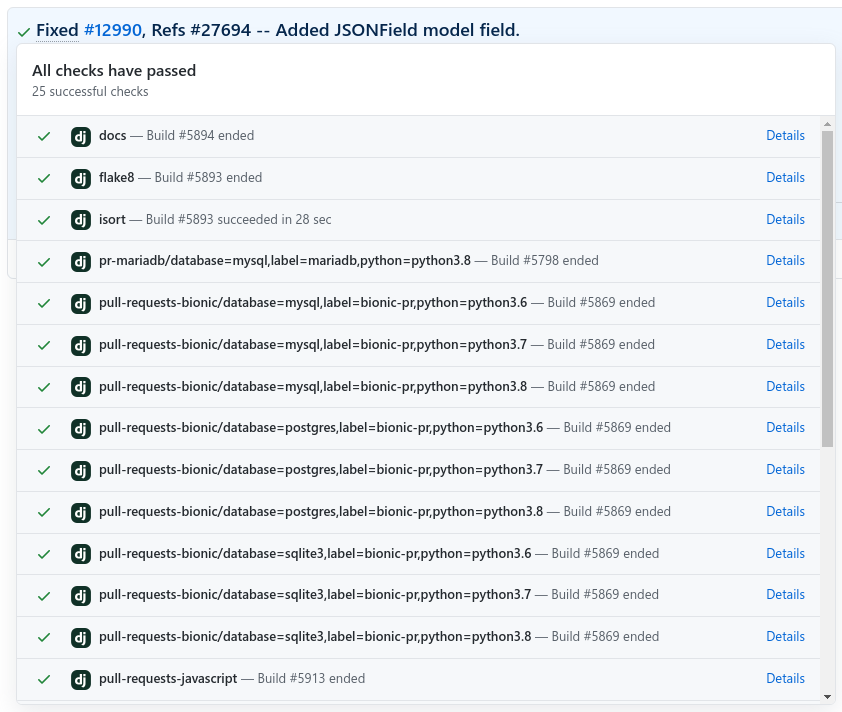
\includegraphics[width=1.00\textwidth]{pics/github-checks.png}
	\caption{The tests have passed on all of the database systems
	(Oracle Database not shown).}
	\label{fig:checks}
\end{figure}

At the time of research, the tests were run on all of the database systems with
Python 3.6, 3.7, and 3.8. The tests were run on Django's Jenkins
instance\footnote{\url{https://djangoci.com}} and the summary that shows the
tests have passed on all of the database systems can be seen on GitHub, as
shown by \autoref{fig:checks}. For Oracle Database, the tests have to be
triggered manually by the Django maintainers. In the final version of the Git
commit, the maintainers did not trigger the tests for Oracle Database, hence
the result cannot be seen in \autoref{fig:checks}. Unfortunately, the build
details and logs for the commit (and the previous iterations) could no longer
be retrieved from the Jenkins instance at the time of writing.
